We present two different case studies that illustrate the results of the refinement algorithm. 

\subsection{Belief liveness + task specification}
Figure \ref{fig:case1} shows a gridworld divided into 'rooms'. The agent needs to patrol the green cell . Additionally, the agent has to constrain the size of its belief of the target location to 3 cells infinitely often. 

\begin{figure}
\centering
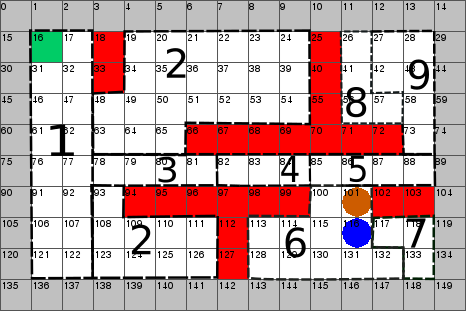
\includegraphics[scale=0.5]{text970.png}\caption{Gridworld with refined 9 abstract states after 5 iterations of refinement.}\label{fig:case1}
\end{figure}

\begin{table}[h!]
\begin{tabular}{c|c|c|c}
& Not refined & Partially refined & Fully refined \\ \hline \hline
Number of states & 104 & 616 & $2\times10^{31}$
\end{tabular}
\end{table}
The refinement algorithm terminates after 5 iterations to produce the refined state shown in figure \ref{fig:case1}. There are 9 belief states which results in an additional 512 states to the full observation game which is far lower than the full reduction which will be a power set of all 104 states.  

 A video simulation can be found at \textbf{LINK}. 

\subsection{Belief safety + task specification}
Figure \ref{fig:case2} shows a 15x20 gridworld that represents an 'outdoor' environment where the red blocks model buildings. In this setting we enforce a belief safety specification in addition to infinitely often reaching the green cell. 